\begin{proof}[Доказательство Теоремы~\ref{thm:II-1} Дирихле]
    По пункту~\ref{lm:II-4-3} Леммы~\ref{lm:II-4} при $\Re{s} > 1$
    \[
        -\frac{L'(s, \chi)}{L(s, \chi)} = \sum_{n=1}^{\infty} \frac{\Lambda(n)\chi(n)}{n^s}.
    \]
    Пусть далее $s = \sigma \in \RR$, $s>1$. Вспомним ещё Определение~\ref{def:I_Mangoldt-function} функции Мангольдта:
    \[
        \Lambda(n) := 
        \begin{cases}
            \ln{p}, & \exists k\colon n = p^k, \\
            0, & \text{иначе}.
        \end{cases}
    \]
    Тогда
    \[
        -\frac{L'(s, \chi)}{L(s, \chi)} = \sum_p \frac{\ln{p} \chi(p)}{p^s} + \sum_p \sum_{k=2}^{\infty} \frac{\ln{p} \chi\left( p^k \right)}{p^{ks}}.
    \]
    Заметим, что первая сумма для $n = p$, а вторая --- для $n = p^k$. Покажем, что второй ряд ограничен некоторой константой, не зависящей от $s$ при $s > 1$:
    \begin{align*}
        \abs{
            \sum_p \sum_{k=2}^{\infty} \frac{\ln{p} \chi\left( p^k \right)}{p^{ks}}
        } &\le \sum_p \sum_{k=2}^{\infty} \frac{\ln{p}}{p^{ks}} = \sum_p \ln{p} \frac{\sfrac{1}{p^2}}{1 - \sfrac{1}{p}} \\
        &\le 2\sum_p \frac{\ln{p}}{p^2} < 2\sum_n \frac{\ln{n}}{n^2} < \infty.
    \end{align*}
    Итак, для любого характера $\chi$ по модулю $m$ мы получили
    \begin{equation}
        \sum_p \frac{\chi(p)\ln{p}}{p^s} = -\frac{L'(s, \chi)}{L(s, \chi)} + \bigO{1}. \tag{$\ast$}\label{eq:II-1}
    \end{equation}
    Поскольку $\gcd{l, m} = 1$, то $\exists v \in \ZZ\colon \congr{vl}{1}{m}$ (то есть обратный). Домножим~(\ref{eq:II-1}) на $\chi(v)$ и просуммируем по всем характерам:
    \[
        \sum_p \frac{\ln{p}}{p^s} \sum_\chi \chi(pv) = -\sum_\chi \chi(v) \frac{L'(s, \chi)}{L(s, \chi)} + \bigO{1}.
    \]
    Вспомним, что из второго пункта Леммы~\ref{lm:II-3}
    \[
        \sum_\chi \chi(pv) =
            \begin{cases}
                \phi(m), & \congr{pv}{1}{m}, \\
                0, & \notcongr{pv}{1}{m}.
            \end{cases}
    \]
    Но $\congr{pv}{1}{m}$, а следовательно, $\congr{p}{l}{m}$, так как $\congr{pl}{1}{m}$.~\newline
    Значит,
    \begin{align*}
        \phi(m) \sum_{\congr{p}{l}{m}} \frac{\ln{p}}{p^s} &= -\sum_\chi \chi(v)\frac{L'(s, \chi)}{L(s, \chi)} + \bigO{1} \\
        \sum_{\congr{p}{l}{m}} \frac{\ln{p}}{p^s} &= -\frac{1}{\phi(m)} \sum_\chi \chi(v)\frac{L'(s, \chi)}{L(s, \chi)} + \bigO{1}.
    \end{align*}
    Перейдём теперь к пределу при $s \to 1+$. Если $\congr{p}{1}{m}$ --- конечное количество, то слева предел конечен. Докажем, что правая же часть стремится к бесконечности (то есть, что в левой части бесконечное число слагаемых):
    \begin{casesp}
        \item
        $\chi \ne \chi_0$. 
            $\frac{L'(s, \chi)}{L(s, \chi)} = \bigO{1}$ при $s \to 1+$.
        \item
        $\chi = \chi_0$.
            $L(s, \chi) = \frac{f(s)}{s - 1}$, где $f(s)$ аналитична в $1$ и $f(1) \ne 0$.
    \end{casesp}
    Значит,
    \[
        \frac{L'(s, \chi_0)}{L(s, \chi_0)} = 
        -\frac{1}{s - 1} + \frac{f'(s)}{f(s)} = 
        -\frac{1}{s - 1} + \bigO{1} \xrightarrow{\text{при } s \to 1+} \infty.
    \]
    То есть мы показали, что правая часть стремится к бесконечности при $s \to 1+$. Следовательно,
    \[
        \sum_{\congr{p}{l}{m}} \frac{\ln{p}}{p^s} = \frac{1}{\phi(m)(s - 1)} + \bigO{1}
    \]
    и Теорема Дирихле полностью доказана.
\end{proof}

\begin{remark}
    Из равенства 
    \[
        \sum_{\congr{p}{l}{m}} \frac{\ln{p}}{p^s} = \frac{1}{\phi(m)(s - 1)} + \bigO{1}
    \]
    можно, в частности, получить, что
    \[
        \sum_p \frac{\ln{p}}{p^s} = \frac{1}{s - 1} + \bigO{1}.
    \]
\end{remark}



\section{Диофантовы приближения}
\label{sec:III_Diophantine-approximations}


\begin{figure}[!ht]
    \centering
    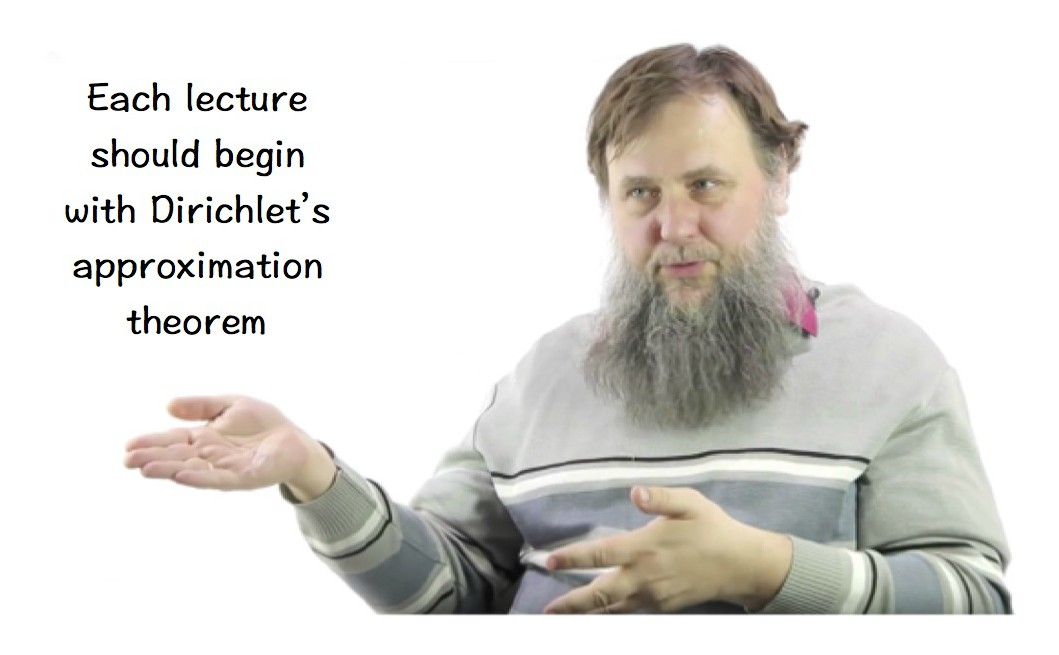
\includegraphics[width=\textwidth]{moschevitin}
    Действительно... Причём лекция может быть по любому предмету.
\end{figure}


\subsection{Предварительные сведения}
\label{subsec:III-1}

Пусть $\theta \in \RR$. Вопрос: насколько маленькой можно сделать разность $\abs{\theta - \frac{p}{q}}$ так, чтобы $\abs{\theta - \frac{p}{q}} < f(a)$ ($p$ и $q$ --- не простые).

\emph{Характеристикой} $\theta$ является то, насколько хорошо она приближается дробью $\frac{p}{q}$. Мы, конечно, знаем, что существуют нерациональные числа ($\sqrt{2}, \sqrt{3}, \dots$). Легко доказать, что корни многочленов с целыми коэффициентами (алгебраические числа, их множество обозначается как \AA) не будут рациональными.

Например, $\phi = \frac{1 + \sqrt{5}}{2}$ --- корень многочлена $x^2 - x - 1 = 0$, а его корни имею вид $\frac{\text{делитель} - 1}{\text{делитель} + 1} \in \{ \pm 1 \}$. Естественно, ни $1$, ни $-1$ корнями не являются.

А вдруг все числа алгебраические? Нет, алгебраических чисел счётное количество. Это доказал Лиувилль через теорию приближений: он показал, что алгебраические числа не могут приближаться ``слишком хорошо''.

То есть, для алгебраических чисел не найдётся такой функции $f$, для которой будет бесконечно много решений.

\begin{nstatement}
\label{stm:III-1}
    Если $\theta = \frac{a}{b} \in \RR$, то
    \[
        \forall \frac{p}{q} \in \QQ \setminus \{ 0 \}\colon \abs{\theta - \frac{p}{q}} > \frac{\sfrac{1}{b}}{q}.
    \]
\end{nstatement}
\begin{proof}
    \[
        \abs{\frac{a}{b} - \frac{p}{q}} = \frac{\abs{aq - bp}}{bq} \ge \frac{1}{bq},
    \] 
    так как $\abs{aq - bp} \in \ZZ\, \ne 0$.
\end{proof}

\begin{ntheorem}[Дирихле о приближении]
\label{thm:III-1}
    Пусть $\theta \in \RR$, $T \in \NN$. Тогда
    \[
        \exists \frac{p}{q} \in \QQ\colon \abs{\theta - \frac{p}{q}} < \frac{1}{qT},
        \quad
        1 \le q \le T.
    \]
\end{ntheorem}
\begin{proof}
    Хотим получить, что $\abs{q\theta - p} < \frac{1}{T}$. Можно считать, что $\theta \in [0, 1)$, и потом просто прибавить целую часть.~\newline
    Рассмотрим числа $\{ n\theta \}$, где $n = 0, 1, \dots, T$. Разобьём отрезок $[0, 1]$ на полуинтервалы $\left[ \frac{k}{T}, \frac{k+1}{T} \right)$, $k = 0, 1, \dots, T-1$ (то есть, на $T$ равных). По принципу Дирихле
    \[
        \exists n_1, n_2\colon 
        \left( n_1 - n_2 \right)\theta - \left( \left[ n_1\theta \right] - \left[ n_2\theta \right] \right) < 
        \frac{1}{T}.
    \]
    Остаётся положить $q = n_1 - n_2$, $p = \left[ n_1\theta \right] - \left[ n_2\theta \right]$. Тогда $q \ge 1$, $q \le T$ (то есть, $n_1, n_2 \le T$).
\end{proof}

\begin{ncorollary}
\label{crl:III-1}
    Если $\theta \in \RR \setminus \QQ$, то неравенство
    \[
        \abs{\theta - \frac{p}{q}} < \frac{1}{q^2}
    \]
    имеет бесконечно много решений в $\frac{p}{q} \in \QQ$.
\end{ncorollary}
\begin{proof}
    Докажем от противного: пусть $\frac{p_1}{q_1}, \frac{p_2}{q_2}, \dots, \frac{p_k}{q_k}$ --- все решения $\abs{\theta - \frac{p}{q}} < \frac{1}{q^2}$. 
    Положим $\delta = \min_i \abs{\theta - \frac{p_i}{q_i}} > 0$, $T = \left\lceil \frac{1}{\delta} \right\rceil$ (любое $T > \frac{1}{\delta}$). 
    По Теореме~\ref{thm:III-1} Дирихле 
    \[
        \exists \frac{p}{q},\, q \le T\colon \abs{\theta - \frac{p}{q}} < \frac{1}{qT} \le \frac{1}{q^2}.
    \]
    То есть $\frac{p}{q}$ должна быть среди дробей $\frac{p_i}{q_i}$. Но
    \[
        \abs{\theta - \frac{p}{q}} < \frac{1}{qT} < \frac{\delta}{q} \le \delta.
    \]
    Таким образом, $\frac{p}{q}$ ``ближе'', чем наименьшее $\delta$ --- пришли к противоречию.
\end{proof}

\begin{ndefinition}
\label{def:III_measure-of-irrationality}
    \emph{Мерой иррациональности} числа $\theta$ называют
    \[
        \mu(\theta) := \sup_s\colon \left\{ \abs{\theta - \frac{p}{q}} < \frac{1}{q^s} \text{ имеет бесконечно много решений } \frac{p}{q} \right\}.
    \]
\end{ndefinition}

\begin{remark}
    В качестве $\frac{p}{q}$ можно брать подходящие дроби в разложении $\theta$ в цепную дробь.
\end{remark}
